\section{Forsøg - Brydningsvinkel}
\subsection{Formål}
Formålet med forsøgene er at undersøge, hvorvidt brydningsloven stemmer overens med virkeligheden. Vi ønsker at finde frem til det ved to delforsøg hvor forsøg 1 handler om at måle brydningsvinkel ved forskellige vinkler, ved anden del forsøg vil vi finde frem til totalrefleksion.

\subsection{Teori}
Når lys går fra et materiale til et andet, vil det brydes, fordi lyset bevæger sig med en forskellig hastighed baseret på hvilket stof det går igennem, dette sker fordi at der er forskellig modstand alt efter hvilket materiale der er tale om, forholdet mellem de to forskellige hastigheder kaldes brydningsindeks. Det kan beregnes ved at bruge formlen: \begin{math}n = \frac{c}{v_{stof}}\end{math}, n er brydningsindeks, c er lysets hastighed og \begin{math}v_{stof}\end{math} er lysets hastighed i et specifikt stof. Brydningsindekset for plexiglas er 1,49 og for luft er brydningsindekset på 1. Hvis man har brug for at udregne brydningsvinklen af lys der går igennem to materialer ved en specifik vinkel kan man bruge formlen: \begin{math}sin(b) = \frac{sin(i)}{n_{2}/n_{1}}\end{math} eller \begin{math}sin(b) = sin(i) \cdot \frac{n_{1}}{n_{2}}\end{math}\newline
Hvor i er indfaldsvinklen, b er brydningsvinklen, n1 er brydningsindekset for stof et og n2 er brydningsindekset for stof to.\newline
Hvis lyset kommer fra et materiale til et andet materiale med en høj brydningsindeks til lav brydningsindeks og hvis vinklen er stor nok, vil der komme en totalrefleksion, som betyder at alt lys bliver reflekteret og ikke går igennem det andet materiale, vinklen kan udregnes ved brug af \begin{math}sin(i_{c}) = \frac{n_{2}}{n_{1}}\end{math}.
\begin{figure}[h!]
    \centering
    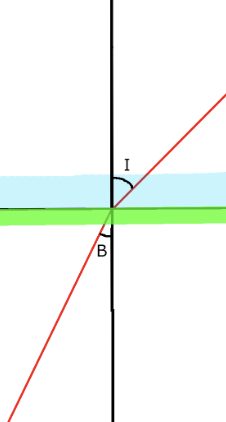
\includegraphics[width=0.25\textwidth]{figures/brydningsvinkeleksempel.png}
    \caption{Eksempel på brydningsvinkel}
\end{figure}
\subsection{Hypotese}
I det at to materialer mødes vil der ske en brydning, det sker fordi lyset skifter hastighed når det går igennem to forskellige materialer, den præcise brydningsvinkel kan beregnes ved brug af \begin{math}\frac{sin(i)}{sin(b)} = \frac{n_{2}}{n_{1}}\end{math} og derfor kan det bevises at formlen passer overens med virkeligheden.\newline
Ved en specifik vinkel, hvis lyset kommer fra et materiale med en høj brydningsindeks til et andet materiale med en lav brydningsindeks vil alt lys blive reflekteret, denne specifikke vinkel kan beregnes ved brug af \begin{math}sin(i_{c}) = \frac{n_{2}}{n_{1}}\end{math} og derfor kan det også vises at denne formel passer overens med virkeligheden.

\subsection{Udstyr}
\begin{itemize}
    \item plexiglas
    \item Papir
    \item Vinkelmåler
    \item Strømforsyning
    \item Lysboks
    \item Blyant
\end{itemize}

\subsection{Fremgangsmåde}
Tegn et stort kryds der går fra midten af alle sider til den modsatte side. Sæt plexiglasset på midten af krydset og tegn rundt om plexiglasset. Sæt plexiglasset lige under en af linjerne på krydset i midten mens den stadig Sæt lysboksen til strømforsyningen og tænd for lysboksen. Lys ind på plexiglasset med en vinkel på 10°.  Husk at lys ind på midten af plexiglasset. Sæt en prik der hvor lysstrålen går ud og mål vinklen. Fortsæt med at øge indfaldsvinklen med 10° indtil du rammer 80°. Mål også 89°.

\subsection{Resultater}
\begin{table}[h]
    \centering
    \begin{tabular}{|c|c|}
        \hline
        Indfaldsvinkel & Brydningsvinkel\\
        \hline
        10 & 6,5\\
        \hline
        20 & 13\\
        \hline
        30 & 19\\
        \hline
        40 & 26\\
        \hline
        50 & 32\\
        \hline
        60 & 37\\
        \hline
        70 & 38\\
        \hline
        80 & 42\\
        \hline
        89 & 43\\
        \hline
    \end{tabular}
\end{table}

I forsøget var der totalrefleksion ved 43 grader

\subsection{Resultatbehandling}
Vi kan starte med at beregne hvornår der vil være en totalrefleksion med formlen nævnt før.
\begin{equation*}
    sin(i_{c}) = \frac{1}{1,49}
\end{equation*}
\begin{equation*}
    sin^{-1}(\frac{1}{1,49}) = i_{c}
\end{equation*}
\begin{equation*}
    i_{c} = 42,155^{\circ}
\end{equation*}

\begin{table}[h]
    \centering
    \begin{tabular}{|c|c|c|c|}
        \hline
        Indfaldsvinkel & Brydningsvinkel Forsøg & Brydningsvinkel Beregnet & Procent Forskel\\
        \hline
        10 & 6,5 & \begin{math}sin^{-1}(sin(10)\cdot \frac{1}{1,49}) = 6,69\end{math} & \begin{math}\frac{6,69 - 6,5}{6,5} \cdot 100 = 2,9\%\end{math}\\
        \hline
        20 & 13 & \begin{math}sin^{-1}(sin(20)\cdot \frac{1}{1,49}) = 13,27\end{math} & \begin{math}\frac{13,27 - 13}{13} \cdot 100 = 2,08\%\end{math}\\
        \hline
        30 & 19 & \begin{math}sin^{-1}(sin(30)\cdot \frac{1}{1,49}) = 19,61\end{math} & \begin{math}\frac{19,61 - 19}{19} \cdot 100 = 3,21\%\end{math}\\
        \hline
        40 & 26 & \begin{math}sin^{-1}(sin(40)\cdot \frac{1}{1,49}) = 25,56\end{math} & \begin{math}\frac{26 - 25,56}{26} \cdot 100 = 1,69\%\end{math}\\
        \hline
        50 & 32 & \begin{math}sin^{-1}(sin(50)\cdot \frac{1}{1,49}) = 30,94\end{math} & \begin{math}\frac{32 - 30,94}{32} \cdot 100 = 3,31\%\end{math}\\
        \hline
        60 & 37 & \begin{math}sin^{-1}(sin(60)\cdot \frac{1}{1,49}) = 35,54\end{math} & \begin{math}\frac{37 - 35,54}{37} \cdot 100 = 3,95\%\end{math}\\
        \hline
        70 & 38 & \begin{math}sin^{-1}(sin(70)\cdot \frac{1}{1,49}) = 39,1\end{math} & \begin{math}\frac{39,1 - 38}{39,1} \cdot 100 = 2,81\%\end{math}\\
        \hline
        80 & 42 & \begin{math}sin^{-1}(sin(80)\cdot \frac{1}{1,49}) = 41,37\end{math} & \begin{math}\frac{42 - 41,37}{42} \cdot 100 = 1,50\%\end{math}\\
        \hline
        89 & 43 & \begin{math}sin^{-1}(sin(89)\cdot \frac{1}{1,49}) = 42,15\end{math} & \begin{math}\frac{43 - 42,14}{43} \cdot 100 = 1,98\%\end{math}\\
        \hline
    \end{tabular}
\end{table}

Procent Gennemsnit
\begin{equation*}
    \frac{2,92\% + 2,08\% + 3,21\% + 1,69\% + 3,31\% + 3,95\% + 2,66\% + 1,50\% + 1,98}{9} = 2,59\%
\end{equation*}

\begin{figure}[htbp]
    \centering
    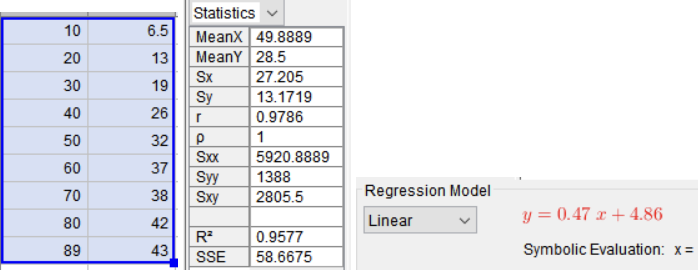
\includegraphics[width=0.7\textwidth]{figures/brydningsvinkelforsoggraf.png}
    \caption{Forsøg data indtastet i GeoGebra}
\end{figure}
\begin{figure}[htbp]
    \centering
    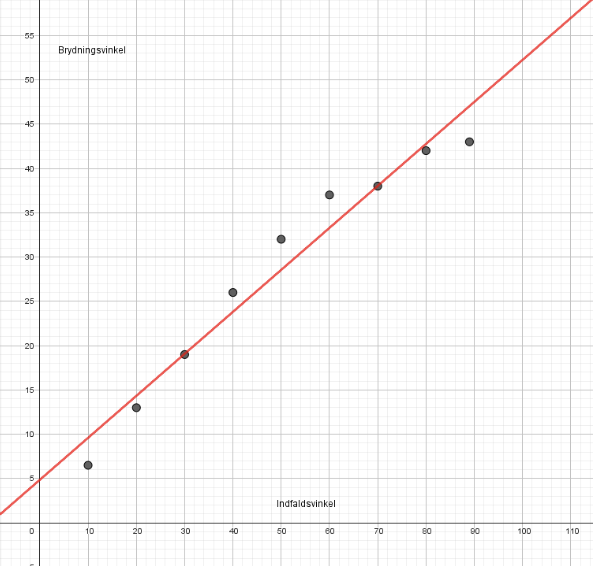
\includegraphics[width=0.6\textwidth]{figures/brydningsvinkelforsoggraf2.png}
    \caption{Graf over forsøgets data}
\end{figure}
\begin{figure}[htbp]
    \centering
    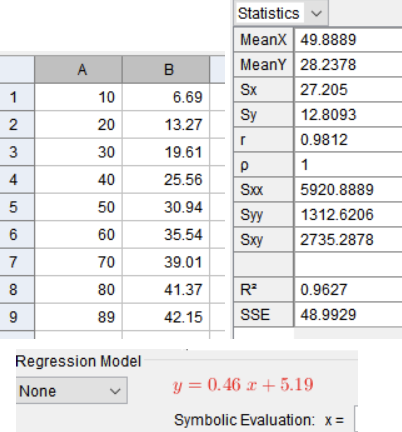
\includegraphics[width=0.45\textwidth]{figures/brydningsvinkelteorigraf.png}
    \caption{Teori data indtastet i GeoGebra}
\end{figure}
\begin{figure}[htbp]
    \centering
    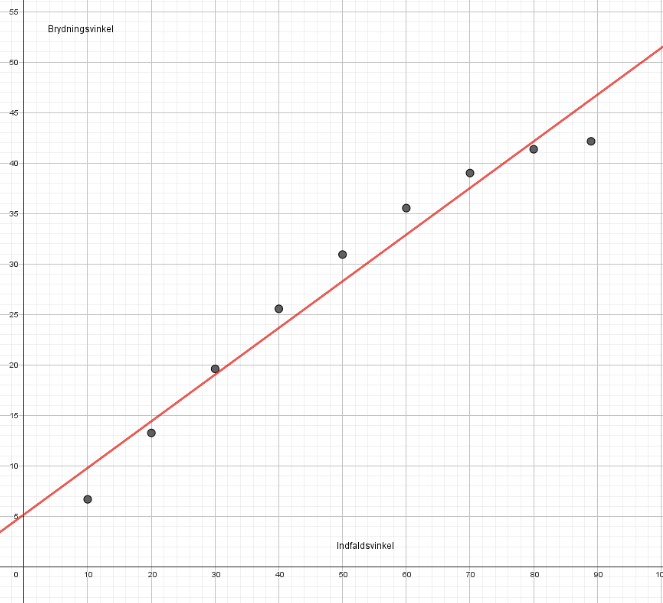
\includegraphics[width=0.6\textwidth]{figures/brydningsvinkelteorigraf2.png}
    \caption{Graf over teoriens data}
\end{figure}
\newpage

\subsection{Diskussion}
Tager man udgangspunkt i graferne og i procent beregningerne kan man se at vores resultater har været rimelig tæt på hvad de skulle have været, inden for de 2,589\% af hvad formlen har sagt det skulle være. Vi tror at den største grund til at vi ikke er tættere er at vi ikke kan måle vinklen helt præcist og det er fordi at det er nok umuligt for et menneske at kunne gøre dette uden instrumenter der kan måle vinklen mere specifikt. Med en R2-værdi på 0,96 kan man godt sige at grafen er sikker dog er der selvfølgelig stadig usikkerhed, i dette tilfælde hvor en grad kan have stor betydning kan det dog stadig godt have en effekt at R2  ikke er tættere på 1. Hvis man kigger på det resultat vi fik til totalrefleksion kan man også se at vi var rimelig tæt på igen, 1,965\% væk fra hvad resultatet ville have været ifølge formlen. Selv om alt det her siger at vi var tætte på at ramme helt rigtigt, kan man ikke endeligt konkludere noget, da der ikke er lavet dobbelt bestemmelse.

\subsection{Konklusion}
Det kan konkluderes i det at 2 materialer mødes, skifter lyset hastighed og derved kan en brydningsvinkel bevises. Det kan derudover konkluderes, at hvis lyset kommer fra et materiale med højt brydningsindeks til et andet materiale med lavt brydningsindeks, vil alt lyset reflekteres også kendt som totalrefleksion. Det kan derfor konkluderes, at de to førnævnte formler stemmer overens med virkeligheden. Dermed er forsøgets formål opnået og kan på baggrund i rapporten. Det skal dog sige at dette ikke er et endegyldigt svar da der som nævnt i diskussionen mangler dobbeltbestemmelse og kontrolforsøg. 